\begin{figure}
	\centering
	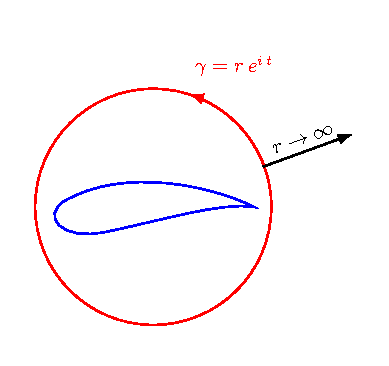
\includegraphics{papers/joukowski/images/04_komplexe_analysis/geschlossenes_linienintegral.pdf}
	\caption{
		Aufgrund der holomorphen Eigenschaft der Funktion kann das Linienintegral um den geschlossenen Kreisbogen $\gamma$,
		welches den Tragflügel komplett umschliesst, gemacht werden.
		Dabei kann der Radius beliebig gross gemacht werden,
		ohne dass sich das Resultat verändert.
		\label{joukowski:komplexe-analysis:fig:geschlossenes-linientintegral}}
\end{figure}
